% A presentation of beamer-floral, written with beamer-floral.
%
% Vector playback needs only the usual build, run from the repository root:
%   latexmk -lualatex -outdir=build/tour docs/src/tour.tex
% For smoother playback, compile with raster samples:
%   python3 tools/build_animation.py --outdir build/tour-raster docs/src/tour-raster.tex
\documentclass[aspectratio=169]{beamer}
\usetheme{floral}
\providecommand\floralplayback{vector}
\usepackage[\floralplayback]{beamer-floral-animation}
\usepackage{hyperref}

\florasetup{seed=3, density=1.2}
\setbeamertemplate{itemize item}[floral]
\setbeamertemplate{itemize subitem}[floral]
\setbeamertemplate{itemize subsubitem}[floral]

\title{beamer-floral}
\subtitle{A garden that grows around your slides}
\author{A tour, written in the package it describes}
\institute{\url{https://github.com/krissen/beamer-floral}}
\date{}

\begin{document}

\florathisframe{growth=timed, growth duration=8, growth fps=20}
\begin{frame}[plain]
  \titlepage
\end{frame}

\section{The idea}

\begin{frame}{Every slide gets its own plant}
  \begin{itemize}
    \item \alert{tikz-flora} draws the flora for each frame.
    \item The text block is measured, so stems grow around it.
    \item A seed makes each garden reproducible.
    \item Blocks and alerts take their colours from the same inks.
  \end{itemize}
  \floraldivider
  \begin{center}
    Text and links stay ordinary, selectable PDF content.
  \end{center}
\end{frame}

\begin{frame}[fragile]{Four lines to start}
\begin{verbatim}
\documentclass{beamer}
\usetheme{floral}
\florasetup{seed=3, density=1.2}
\begin{document} ... \end{document}
\end{verbatim}
  Compile with LuaLaTeX. \texttt{latexmk} runs the passes that settle the
  measured geometry.
\end{frame}

\section{Inks}

\begin{frame}{The warm palette}
  \begin{block}{Gold hero, warm blooms}
    The default: a gold hero, warm blooms and earth foliage.
  \end{block}
  \begin{alertblock}{Alerts}
    \alert{Alerts} take a deeper ink from the same family.
  \end{alertblock}
  \begin{exampleblock}{Examples}
    Examples follow the foliage.
  \end{exampleblock}
\end{frame}

\florapalette{blue}
\begin{frame}{The blue palette}
  \begin{block}{Blooms and leaves in blue}
    \texttt{\textbackslash florapalette\{blue\}} changes the flora and the theme.
  \end{block}
  \begin{alertblock}{Alerts}
    \alert{Alerts} move to violet.
  \end{alertblock}
\end{frame}

\florapalette{green}
\begin{frame}{The green palette}
  \begin{block}{Blue blooms, green leaves}
    \texttt{green-stems} also colours the stems.
  \end{block}
  \begin{exampleblock}{Examples}
    Examples take the leaf green.
  \end{exampleblock}
\end{frame}
\florapalette{warm}

\florathisframe{palette={hero=kon-peki, blooms=warm, leaves=teal}}
\begin{frame}[fragile]{Or mix your own}
\begin{verbatim}
\florasetup{palette={hero=kon-peki,
  blooms=warm, leaves=teal}}
\end{verbatim}
  A custom palette changes the flora. Set theme colours yourself with
  \texttt{\textbackslash setbeamercolor}.
\end{frame}

\section{Composition}

\florathisframe{layout=left}
\begin{frame}{Layout: left}
  The border fills the left margin, the top and the foot.\par\medskip
  The right margin stays paper.
\end{frame}

\florathisframe{layout=surround}
\begin{frame}{Layout: surround}
  The crown stops under the running head and the foot closes the border.
\end{frame}

\florathisframe{density=0.5}
\begin{frame}{Density 0.5: more paper}
  Fewer stems and blooms, the same measured text block.
\end{frame}

\florathisframe{density=2.2}
\begin{frame}{Density 2.2: a fuller margin}
  More growth, and the text is still left alone.
\end{frame}

\florathisframe{density=0.8, mix={leaves=3, bloom=0, soft=0, lily=0,
  ghost=0, umbel=0, cyme=0, gyps=0}}
\begin{frame}{A quiet, foliage-led mix}
  \texttt{mix=\{\ldots\}} weighs the parts of the garden against each other.
\end{frame}

\florathisframe{visitors=2}
\begin{frame}{Visitors}
  \texttt{visitors} adds bees, butterflies, birds and snails.\par\medskip
  Keep them sparse in a real talk.
\end{frame}

\florathisframe{seed=11}
\begin{frame}{Another seed, another garden}
  \texttt{seed} is a number, or \texttt{random}.\par\medskip
  The same seed and text give the same plant on every build.
\end{frame}

\section{Growth}

\florathisframe{growth=overlays}
\begin{frame}{Growth across overlays}
  \begin{itemize}
    \item Each click reveals more of the garden.\pause
    \item Stems extend before their leaves.\pause
    \item Leaves and flowers open as whole shapes.\pause
    \item The last overlay is the finished plant.
  \end{itemize}
\end{frame}

\florathisframe{growth=timed, growth duration=6, growth fps=20}
\begin{frame}{Timed growth}
  \begin{itemize}
    \item Each overlay plays its own interval.\pause
    \item Time spent waiting between clicks is not counted.\pause
    \item Printed pages and handouts show the finished flora.
  \end{itemize}
\end{frame}

\begin{frame}{Three kinds of growth}
  \begin{description}
    \item[off] A static garden, the default.
    \item[overlays] A manual reveal as you step through the slide.
    \item[timed] An animation, for viewers that can play it.
  \end{description}
  \floraldivider
  \begin{center}\small
    Vector playback needs only LaTeX. Raster playback is smoother and
    needs Python and Poppler at build time.
  \end{center}
\end{frame}

\section{Details}

\floralornamentsetup{item=rosette, subitem=gilt_trefoil, subsubitem=gilt_lozenge}
\begin{frame}{Ornaments in lists}
  \begin{itemize}
    \item A pointed rosette at the first depth.
      \begin{itemize}
        \item A trefoil below it.
          \begin{itemize}
            \item A lozenge for the finest detail.
          \end{itemize}
      \end{itemize}
  \end{itemize}
\end{frame}
\floralornamentsetup{item=gilt_rosette, subitem=gilt_rosette, subsubitem=gilt_rosette}

\begin{frame}{Dividers}
  The default is a fleuron rule.
  \floraldivider
  \floralornamentsetup{divider=swash, divider width=.35\linewidth,
    divider color=florastructure}
  A shorter swash in the accent ink.
  \floraldivider
  \floralornamentsetup{divider=headpiece, divider width=.7\linewidth,
    divider height=1.2em, divider color=floraexample}
  A wider headpiece in the example ink.
  \floraldivider
\end{frame}

\florareserve{0pt}{0pt}{\the\paperwidth}{\the\dimexpr 1.2cm\relax}
\florabackground[bottom]{florablockbody}{1.2cm}
\begin{frame}{Reserving space}
  \texttt{\textbackslash florareserve} keeps the flora out of a rectangle.\par\medskip
  \texttt{\textbackslash florabackground} adds a band beneath it: room for a
  footline, a logo or a caption.
\end{frame}
\floraclearreserve
\florabackground[bottom]{white}{0pt}

\begin{frame}[allowframebreaks=0.72]{Long frames keep growing}
  Continuation pages each get their own garden.
  \begin{itemize}
    \item One idea per line, as in a real talk.
    \item Another idea, to take up some room.
    \item A third, measured like the others.
    \item A fourth.
    \item A fifth.
    \item A sixth.
    \item A seventh.
    \item An eighth, to force a new page.
    \item A ninth.
    \item A tenth.
    \item An eleventh.
    \item A twelfth.
    \item A thirteenth.
    \item A fourteenth, on the last page.
  \end{itemize}
\end{frame}

\section{Working with others}

\begin{frame}{Beside a stock theme}
  \begin{columns}[c,onlytextwidth]
    \begin{column}{.55\textwidth}
      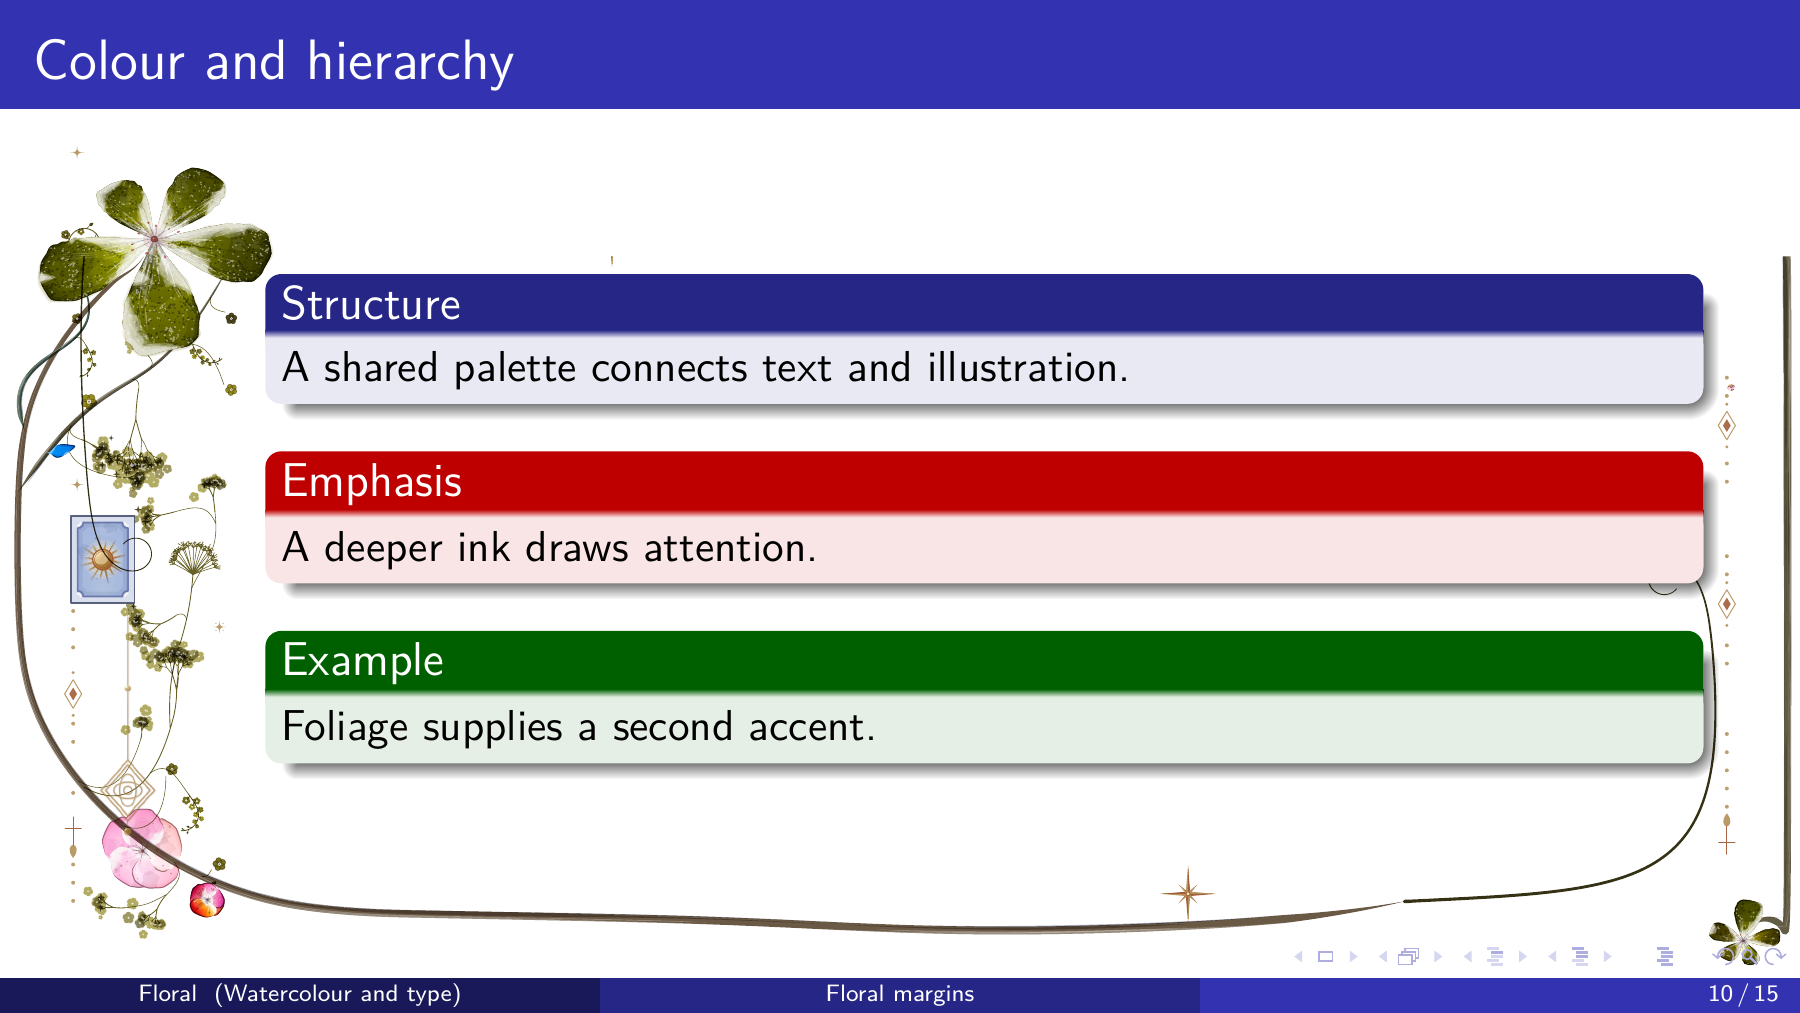
\includegraphics[width=\linewidth]{docs/img/stock-madrid.png}
    \end{column}
    \begin{column}{.42\textwidth}\small
      Load the theme first, then \texttt{beamer-floral}. The flora starts
      below the title and the theme keeps its colours.
    \end{column}
  \end{columns}
\end{frame}

\floraoff
\begin{frame}{Flora off}
  \texttt{\textbackslash floraoff} leaves a frame undecorated, for a dense
  table or a full-width figure.
\end{frame}
\floraon

\section{Closing}

\begin{frame}[label=garden]{Requirements and limits}
  \begin{itemize}
    \item LuaLaTeX only.
    \item Keep floral settings constant within one frame.
    \item Timed growth needs a PDF viewer that plays it, such as Acrobat Reader.
    \item Files are large: a 21-page test deck is 22~MB static and 68~MB with
      vector growth.
  \end{itemize}
\end{frame}

\againframe{garden}

\florathisframe{layout=left, density=2}
\begin{frame}{Plant your own}
  \begin{center}
    \url{https://github.com/krissen/beamer-floral}\par\bigskip
    Built on \href{https://github.com/wn-mitch/tikz-flora}{tikz-flora}.
  \end{center}
\end{frame}

\end{document}
